% Schema of the fin10k knowledge graph. Compile on its own (pdflatex schema_figure.tex) to get
% schema_figure.pdf, then \includegraphics it in the report.
\documentclass[tikz,border=4pt]{standalone}
\usetikzlibrary{arrows.meta,positioning,fit,backgrounds}
\begin{document}
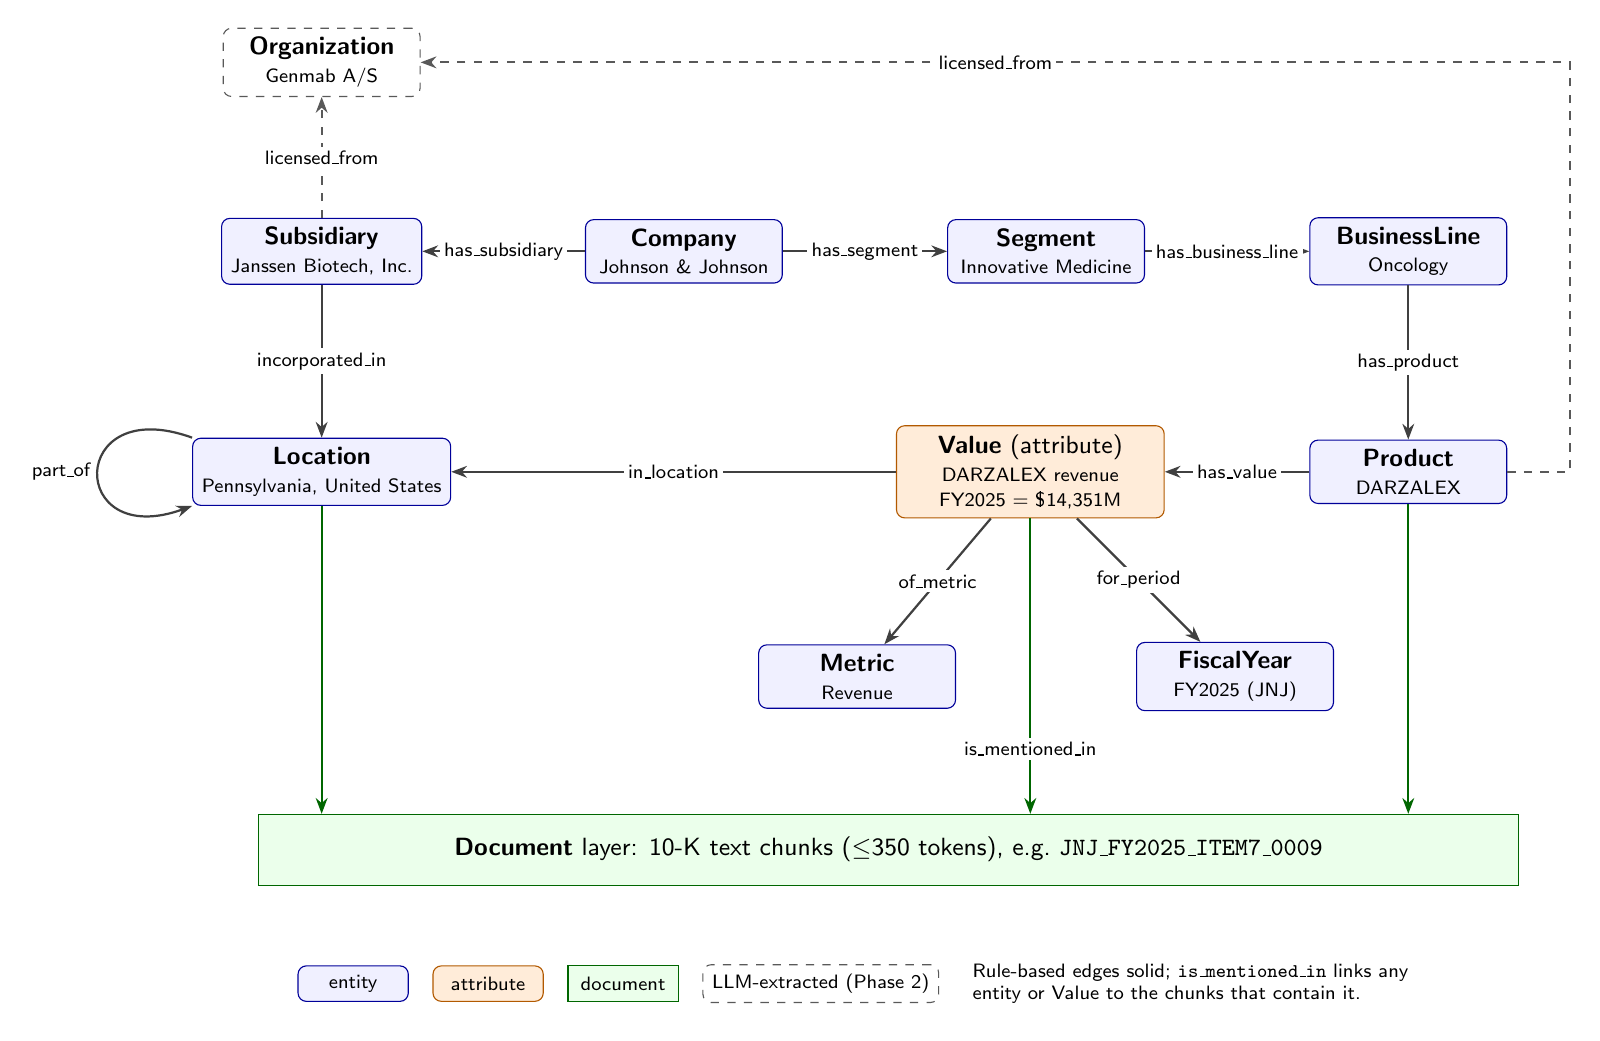
\begin{tikzpicture}[
  font=\sffamily\small,
  >={Stealth[length=2mm]},
  ent/.style={draw=blue!60!black, fill=blue!6, rounded corners=3pt, minimum width=2.5cm,
              minimum height=0.8cm, align=center},
  att/.style={draw=orange!70!black, fill=orange!15, rounded corners=3pt, minimum width=2.5cm,
              minimum height=0.8cm, align=center},
  llm/.style={draw=gray!70!black, dashed, fill=white, rounded corners=3pt, minimum width=2.5cm,
              minimum height=0.8cm, align=center},
  doc/.style={draw=green!40!black, fill=green!8, minimum height=0.9cm, align=center},
  rel/.style={->, thick, draw=black!75},
  rell/.style={->, thick, dashed, draw=gray!70!black},
  lab/.style={font=\sffamily\scriptsize, fill=white, inner sep=1.5pt},
]
% ---- entity layer
\node[ent] (comp) at (0,0)      {\textbf{Company}\\[-1pt]\scriptsize Johnson \& Johnson};
\node[ent] (sub)  at (-4.6,0)   {\textbf{Subsidiary}\\[-1pt]\scriptsize Janssen Biotech, Inc.};
\node[ent] (loc)  at (-4.6,-2.8){\textbf{Location}\\[-1pt]\scriptsize Pennsylvania, United States};
\node[ent] (seg)  at (4.6,0)    {\textbf{Segment}\\[-1pt]\scriptsize Innovative Medicine};
\node[ent] (bl)   at (9.2,0)    {\textbf{BusinessLine}\\[-1pt]\scriptsize Oncology};
\node[ent] (prod) at (9.2,-2.8) {\textbf{Product}\\[-1pt]\scriptsize DARZALEX};
\node[ent] (met)  at (2.2,-5.4) {\textbf{Metric}\\[-1pt]\scriptsize Revenue};
\node[ent] (fy)   at (7.0,-5.4) {\textbf{FiscalYear}\\[-1pt]\scriptsize FY2025 (JNJ)};
% ---- attribute layer
\node[att, minimum width=3.4cm] (val) at (4.4,-2.8)
     {\textbf{Value} (attribute)\\[-1pt]\scriptsize DARZALEX revenue\\[-2pt]\scriptsize FY2025 = \$14,351M};
% ---- phase 2 (LLM)
\node[llm] (org) at (-4.6,2.4) {\textbf{Organization}\\[-1pt]\scriptsize Genmab A/S};

% ---- rule-based relations
\draw[rel] (comp) -- node[lab]{has\_subsidiary} (sub);
\draw[rel] (sub)  -- node[lab]{incorporated\_in} (loc);
\draw[rel] (loc.north west) to[out=160,in=200,looseness=5] node[lab, left=1pt]{part\_of} (loc.south west);
\draw[rel] (comp) -- node[lab]{has\_segment} (seg);
\draw[rel] (seg)  -- node[lab]{has\_business\_line} (bl);
\draw[rel] (bl)   -- node[lab]{has\_product} (prod);
\draw[rel] (prod) -- node[lab]{has\_value} (val);
\draw[rel] (val)  -- node[lab]{of\_metric} (met);
\draw[rel] (val)  -- node[lab]{for\_period} (fy);
\draw[rel] (val)  -- node[lab]{in\_location} (loc);

% ---- phase 2 relations
\draw[rell] (sub)  -- node[lab]{licensed\_from} (org);
\draw[rell] (prod.east) -- ++(0.8,0) |- node[lab, pos=0.75]{licensed\_from} (org.east);

% ---- document layer
\node[doc, minimum width=16cm] (docs) at (2.6,-7.6)
  {\textbf{Document} layer: 10-K text chunks ($\leq$350 tokens), e.g.\ \texttt{JNJ\_FY2025\_ITEM7\_0009}};
\draw[rel, draw=green!40!black] (val.south) -- node[lab, pos=0.78]{is\_mentioned\_in} (val.south |- docs.north);
\draw[rel, draw=green!40!black] (loc.south) -- (loc.south |- docs.north);
\draw[rel, draw=green!40!black] (prod.south) -- (prod.south |- docs.north);

% ---- legend
\node[ent, minimum width=1.4cm, minimum height=0.45cm, font=\sffamily\scriptsize] (l1) at (-4.2,-9.3) {entity};
\node[att, minimum width=1.4cm, minimum height=0.45cm, font=\sffamily\scriptsize, right=0.3cm of l1] (l2) {attribute};
\node[doc, minimum width=1.4cm, minimum height=0.45cm, font=\sffamily\scriptsize, right=0.3cm of l2] (l3) {document};
\node[llm, minimum width=2.6cm, minimum height=0.45cm, font=\sffamily\scriptsize, right=0.3cm of l3] (l4) {LLM-extracted (Phase 2)};
\node[font=\sffamily\scriptsize, right=0.3cm of l4, align=left] {Rule-based edges solid; \texttt{is\_mentioned\_in} links any\\entity or Value to the chunks that contain it.};
\end{tikzpicture}
\end{document}
